\documentclass[a4paper]{article}
\usepackage[utf8]{inputenc}
\usepackage{amsmath}
\usepackage{amssymb}
\usepackage{caption}
\usepackage{mathtools}
\usepackage{amsfonts}
\usepackage{lastpage}
\usepackage{tikz}
\usepackage{float}
\usepackage{textcomp}
\usetikzlibrary{patterns}
\usepackage{pdfpages}
\usepackage{gauss}
\usepackage{fancyvrb}
\usepackage[table]{colortbl}
\usepackage{fancyhdr}
\usepackage{graphicx}
\usepackage[margin=2.5 cm]{geometry}

\definecolor{listinggray}{gray}{0.9}
\usepackage{listings}
\lstset{
	language=,
	literate=
		{æ}{{\ae}}1
		{ø}{{\o}}1
		{å}{{\aa}}1
		{Æ}{{\AE}}1
		{Ø}{{\O}}1
		{Å}{{\AA}}1,
	backgroundcolor=\color{listinggray},
	tabsize=3,
	rulecolor=,
	basicstyle=\scriptsize,
	upquote=true,
	aboveskip={0.2\baselineskip},
	columns=fixed,
	showstringspaces=false,
	extendedchars=true,
	breaklines=true,
	prebreak =\raisebox{0ex}[0ex][0ex]{\ensuremath{\hookleftarrow}},
	frame=single,
	showtabs=false,
	showspaces=false,
	showlines=true,
	showstringspaces=false,
	identifierstyle=\ttfamily,
	keywordstyle=\color[rgb]{0,0,1},
	commentstyle=\color[rgb]{0.133,0.545,0.133},
	stringstyle=\color[rgb]{0.627,0.126,0.941},
  moredelim=**[is][\color{blue}]{@}{@},
}

\lstdefinestyle{base}{
  emptylines=1,
  breaklines=true,
  basicstyle=\ttfamily\color{black},
}

\pagestyle{fancy}
\def\checkmark{\tikz\fill[scale=0.4](0,.35) -- (.25,0) -- (1,.7) -- (.25,.15) -- cycle;}
\newcommand*\circled[1]{\tikz[baseline=(char.base)]{
            \node[shape=circle,draw,inner sep=2pt] (char) {#1};}}
\newcommand*\squared[1]{%
  \tikz[baseline=(R.base)]\node[draw,rectangle,inner sep=0.5pt](R) {#1};\!}
\newcommand{\comment}[1]{%
  \text{\phantom{(#1)}} \tag{#1}}
\newcommand{\pd}[2]{%
  \frac{\partial^{#2}}{\partial #1^{#2}}}
\def\el{[\![}
\def\er{]\!]}
\def\dpip{|\!|}
\def\MeanN{\frac{1}{N}\sum^N_{n=1}}
\cfoot{Page \thepage\ of \pageref{LastPage}}
\DeclareGraphicsExtensions{.pdf,.png,.jpg}
\author{Nikolaj Dybdahl Rathcke (rfq695) \\
        Victor Petren Bach Hansen (grn762) \\
        Tobias Hallundbæk Petersen (xtv657) }
\title{Signal and Image Processing \\ Assignment 4}
\lhead{SIP}
\rhead{Assignment 4}

\begin{document}
\maketitle
\section*{Question 1}
The code for this question is seen below:
\lstinputlisting[language=Matlab]{src/q1.m}
We want to show that a convolution of a gaussian with itself is also gaussian by calculating images from its scale-space. The filter \texttt{A} is a gaussian kernel with sigma equal to the parameter $s$, which is $3$. To calculate an image from its scale space, we use the handed out \texttt{scale} with parameter $t=4$, called tau. The other image is calculated directly using $\sigma=\sqrt{s^2+t^2}$. The output from running the file is two images, which are shown in Figure \ref{q1_1}.
\begin{figure}[H]
  \centering
  \captionsetup{justification=centering}
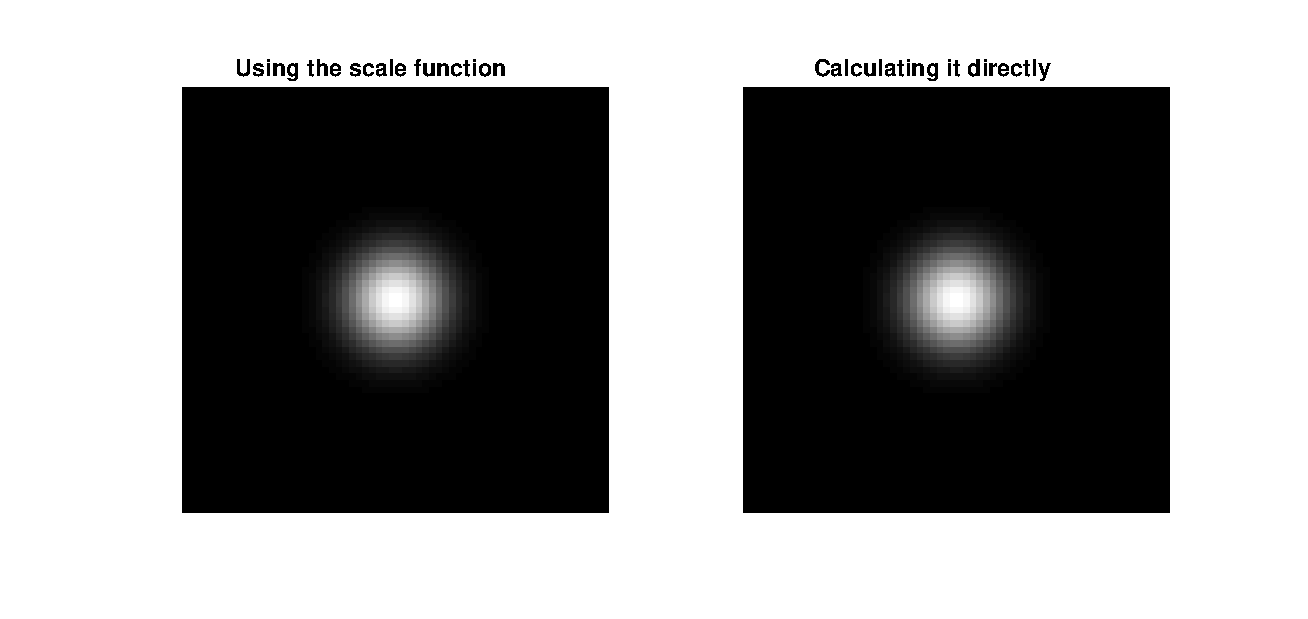
\includegraphics[width=\textwidth]{q1_1.eps}
  \caption{Figure showing the resulting images from calculating a convolution of a gaussian with itself by its scale space and directly.}
  \label{q1_1}
\end{figure}
Even though the images seem to be identical, this is not the case. However, the error is very small. The mean squared error between the two approaches is $2.3440\cdot10^{-25}$, so the images are very similar.

\section*{Question 2}
\subsection*{(a)}
We want to calculate the analytical expression for $H(x,y,\tau)$ for $\gamma = 1$.
\begin{align*}
  H(x,y,\tau) &= I_{xx}(x,y,\tau) + I_{yy}(x,y,\tau)\\
  &= \tau^2 \left( \pd{x}{2} I(x,y,\tau) \pd{y}{2} I(x,y,\tau) \right) \comment{Using (5)}\\
  &= \tau^2 \left( \pd{x}{2} G(x,y,\sqrt{\tau^2 + \sigma^2}) + \pd{y}{2} G(x,y,\sqrt{\tau^2 + \sigma^2})\right) \comment{Using (2), (3) and (4)}\\
  &= \tau^2 \left( \pd{x}{2} \left(\frac{1}{2\pi(\tau^2 + \sigma^2)}e^{-\frac{x^2 + y^2}{2(\tau^2 + \sigma^2)}}\right) + \pd{y}{2} \left(\frac{1}{2\pi(\tau^2 + \sigma^2)}e^{-\frac{x^2 + y^2}{2(\tau^2 + \sigma^2)}}\right) \right) \comment{Using (1)}\\
  &= \tau^2 \left(\frac{2x^2e^{- \frac{x^2+y^2}{2\sigma^2 +2\tau^2}}}{(2\sigma^2 + 2\tau^2)^2\pi(\sigma^2 + \tau^2)}- \frac{e^{- \frac{x^2+y^2}{2\sigma^2 +2\tau^2}}}{(2\sigma^2 + 2\tau^2)\pi(\sigma^2 + \tau^2)}\right) + \\
  &\phantom{=} \tau^2\left(\frac{2y^2e^{- \frac{x^2+y^2}{2\sigma^2 +2\tau^2}}}{(2\sigma^2 + 2\tau^2)^2\pi(\sigma^2 + \tau^2)}- \frac{e^{- \frac{x^2+y^2}{2\sigma^2 +2\tau^2}}}{(2\sigma^2 + 2\tau^2)\pi(\sigma^2 + \tau^2)}\right) \comment{Deriving the expression twice}\\
  &= - \frac{t^2 e^{-\frac{x^2 + y^2}{2\sigma^2 + 2\tau^2}}(2\sigma^2 + 2 \tau^2 - x^2 - y^2)}{2(\sigma^2 + \tau^2)^3 \pi} \comment{Simplified}
\end{align*}
Which is the analytical expression for $H(x,y,\tau)$.
\subsection*{(b)}
We here set $x=y=0$ in the analytical expression resulting in the following:
$$
H(0,0,\tau) = \frac{-2\tau^2}{(2\sigma^2 + 2 \tau^2)\pi(\sigma^2 + \tau^2)}
$$
To find the extremal point it is first differentiated
\begin{align*}
  \pd{\tau}{}H(0,0,\tau) &= \pd{\tau}{} \left(\frac{-2\tau^2}{(2\sigma^2 + 2 \tau^2)\pi(\sigma^2 + \tau^2)}\right)\\
  &= \frac{2(\tau^3 -\sigma^2 \tau)}{\pi(\sigma^2 + \tau^2)^3}
\end{align*}
Setting this to 0 and solving for $\tau$ results in the three solutions: $0, \sigma, -\sigma$. We can see that the value of the scale normalized image of the Laplacian is extremal for $\tau = 0$. Changing $\tau$ to values close to $\sigma$ results in a negative expression, meaning that the function decreases in value around $\tau = \sigma$.
\subsection*{(c)}
We confirm this in Matlab using the following code:
\lstinputlisting[firstline=0,lastline=9,language=MATLAB]{./src/q2.m}
Which results in Figure \ref{2c}, where it can easily be seen that it confirms what was concluded in the above subquestion.
\begin{figure}[H]
  \centering
  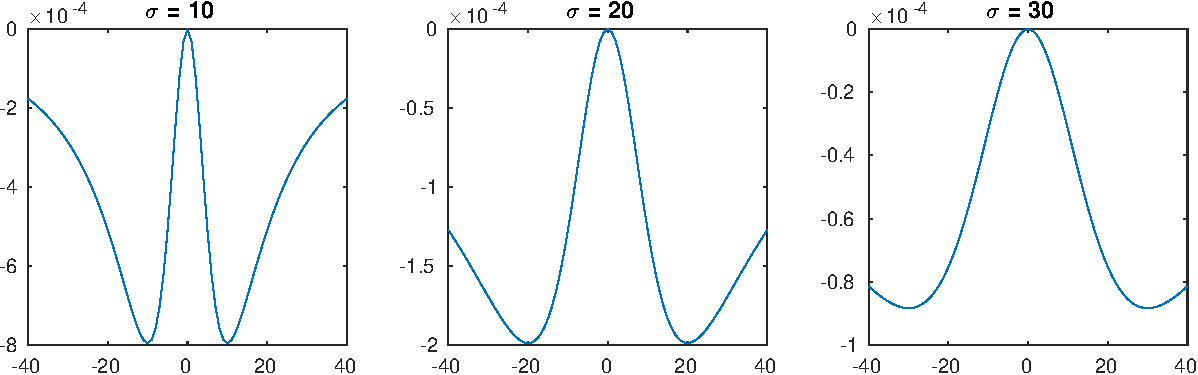
\includegraphics[width=0.8\textwidth]{./2c.pdf}
  \caption{$H(0,0,\tau)$ plotted with $\sigma \in {10,20,30}$.}
  \label{2c}
\end{figure}

\subsection*{(d)}
To do blob detection using Laplacian of Gaussian we must first create the filtered images at different scales, we have chosen $\sigma = \{15,17...33,35\}$. We here chose for each filtering a window of size $\sigma*6 + 1$ as this produced the best results. This is done using the following Matlab function:
\lstinputlisting[language=MATLAB]{./src/scaleSpace.m}
After these are created we compare each value with its six neighbours in the scale space, the four in the same scale, and the one above and below. If the value is greater than its neighbours it must be a local maxima, the 20 highest of these are saved. This is done in the  Matlab function \texttt{nMax} (omitted as it is rather long).\\
%\lstinputlisting[language=MATLAB]{./src/nMax.m}
To find bright spots the image is inverted, but otherwise the procedure is the same. The functions are combined in the following Matlab code:
\lstinputlisting[firstline=10,lastline=25,language=MATLAB]{./src/q2.m}
Which produces the image seen in Figure \ref{2d}, we can see that it had high success in detecting the blobs. A lot of the blobs are overlapping, this could possibly be improved by making some restriction on how close they can be.
\begin{figure}[H]
  \centering
  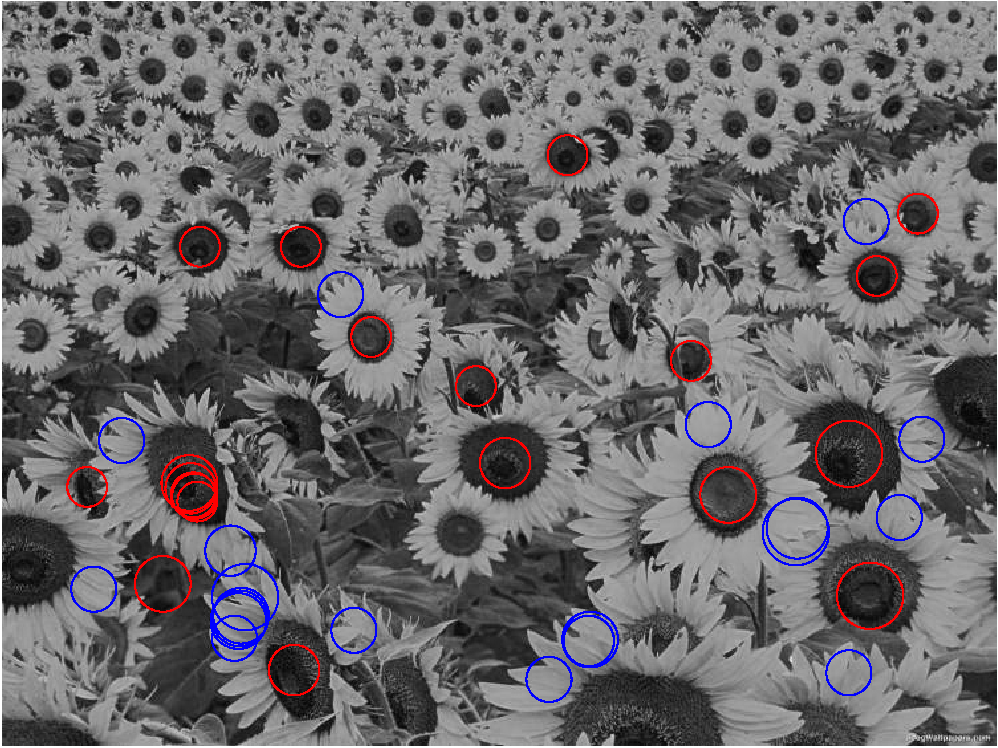
\includegraphics[width=0.8\textwidth]{./2d.pdf}
  \caption{Blob detection using Laplacian of Gaussian, red circles represent dark spots and blue represent bright spots}
  \label{2d}
\end{figure}
\section*{Question 3}
\subsection*{(a)}
When having a soft edge defnied as following:
$$
  J(x,y)=\int^{x}_{-\infty} G(x',0,\sigma)dx'
$$
where its scale-space is defined as following:
$$
  J(x,y,\tau)=J(x,y)**G(x,y,\tau)
$$
Finding the $x$ and $y$ components of this is done as following. $J_x$ is found by taking the derivative of $J(x,y,\tau)$ w.r.t. $x$. As $J(x,y)$ is expressed as an integral, taking the derivative cancels it out, leaving the body of the integral:
\begin{align*}
  J_x &= \frac{\partial}{\partial x}(J(x,y) ** G(x,y,\tau)) \\
      &= \frac{\partial}{\partial x} (J(x,y)) ** G(x,y,\tau) \\
      &= G(x,0,\sigma) ** G(x,y,\tau)
\end{align*}
We can apply the same procedure for $J_y$, but as the y-component of the integral body is $0$, $J_y$ will be zero aswell:
\begin{align*}
  J_y &= \frac{\partial}{\partial y}(J(x,y) ** G(x,y,\tau)) \\
      &= 0
\end{align*}
we can therefore disregard $J_y$. The Gaussian kernel, $G(x,y,\tau)$, can be expreseed analytically by using equation (1):
$$
  G(x,y,\tau) = \frac{1}{2\pi \tau^2} e^{-\frac{x^2+y^2}{2\tau^2} }
$$
which now can be expressed in terms of the one-dimensional Gaussian kernel:
\begin{align*}
  G(x,y,\tau) &= \frac{1}{2\pi \tau^2} e^{-\frac{x^2+y^2}{2\tau^2} } \\
              &= \frac{1}{2\pi \tau^2} e^{-\frac{x^2}{2\tau^2} } e^{-\frac{y^2}{2\tau^2} }\\
              &= \frac{1}{\sqrt{2\pi \tau^2}} e^{-\frac{x^2}{2\tau^2} } \frac{1}{\sqrt{2\pi \tau^2}} e^{-\frac{y^2}{2\tau^2} }\\
              &= G(x,\tau)G(y,\tau)
\end{align*}
Now we can write $J_x$ where the integration only is done over one part of the expression
$$
J_x = \int_{-\infty}^{\infty}\int_{-\infty}^{\infty} G(x', 0,\tau) G(x-x',\tau) \:dx' \: G(y-y')\: dy'
$$
In order to simpify this expression, the following two observations can be used.

First of all, it can be seen that the integral of the $y$-component multiplied by any constant $k$,  will result in $k$, which removed the integral over this $y$-component:
$$
  \int^{\infty}_{-\infty} k G(y-y',\tau)\:dy' = k
$$
And secondly, we can use a modification of equation (2) for one dimension only, and the convolution can be expressed as:
$$
  G(x',0,\sigma)**G(x-x',\tau) = \hat{G}(x,\sqrt{\sigma^2 + \tau^2})
$$
which means we now can express $J_x$ as
$$
  J_x = \hat{G}(x,\sqrt{\sigma^2 +\tau^2})
$$
Here, $\hat{G}$ is the normalized expression for $G$, found the following way:
\begin{align*}
  G(x,0,\sigma) &= \frac{1}{2\pi\sigma^2}e^{-\frac{x^2}{2\sigma^2} } \\
                &= \frac{1}{\sqrt{2\pi\sigma^2}} (G(x,\sigma))\\
                &= \hat{G}(x,\sqrt{\sigma^2, \tau^2})
\end{align*}
Now that we have found $J_x$, the scale normalized derivative $J_x'$ must be found, which is done by using $\gamma = \frac{1}{2} $ $i=1$ and $j=0$ in equation (5):
$$
J_x' = \sqrt{\tau}J_x
$$
We can use this in equation (9) and get the desired analytical expression:
\begin{align*}
  |\!| \nabla I |\!|^2 &= J_x^2 + J_y^2\\
                       &= \tau (J_x^2 + J_y^2)\\
                       &= \tau \left( \frac{1}{\sqrt{ 2\pi\sigma^2}}G(x,\sqrt{\sigma^2 + \tau^2})  \right)\\
                       &= \frac{\tau}{\sqrt{2\pi\sigma^2}} \frac{1}{2\pi(\sigma^2 + \tau^2)} e^{- \frac{x^2}{2(\sigma^2 + \tau^2)} } \comment{last factor subst from eq (1)}
\end{align*}

\subsection*{(b)}
We can find the scale for which the point in $(0,0)$ is maximal, by taking the derivative of the analytical expression found previously (with $x=0$):
$$
\frac{\tau}{\sqrt{2\pi\sigma^2}} \frac{1}{2\pi(\sigma^2 + \tau^2)} e^{- \frac{x^2}{2(\sigma^2 + \tau^2)} } = \frac{\tau}{\sqrt{2\pi\sigma^2}} \frac{1}{2\pi(\sigma^2 + \tau^2)}
$$
We take the derivative of this expression w.r.t. $\tau$ and get:
$$
\frac{\partial}{\partial \tau} \frac{\tau}{\sqrt{2\pi \sigma^2}} \frac{1}{2\pi(\sigma^2 + \tau^2)} = \frac{\sigma^2-\tau^2}{2\pi^{3/2}\sqrt{2\sigma^2}(\sigma^2+x^2)^2}
$$
Even though this can be simplied, it is easy to see there is a maximum at $\tau=\sigma$ (we disregard the negative value of $\tau$) as the numerator becomes $0$, which means the entire expression is $0$. This is not a maximum in $(x, y, \tau)$ though. The exponential term will contribute to the numerator, as the product rule states that $(f\cdot g)'=f'\cdot g + f\cdot g$. By actually making the derivation, we can verify this:
$$
\frac{\partial}{\partial \tau} \frac{\tau}{\sqrt{2\pi \sigma^2}} \frac{1}{2\pi(\sigma^2 + \tau^2)} e^{-\frac{x}{2(\sigma^2+\tau^2)}} = \frac{e^{-\frac{x^2}{2(\sigma^2+\tau^2)}}(\sigma^4-\tau^2(\tau^2-2x))}{2\sqrt{2}\pi^{3/2}\sqrt{\sigma^2}(\sigma^2+\tau^2)^3}
$$
This means that when we cannot pick a value for $\tau$ to make the expression $0$ and find the maxima as it depends on $x$ and $\sigma$.

\subsection*{(c)}
In the same fashion as (c) in Question $2$, we use the following Matlab code to confirm it:
\lstinputlisting[language=Matlab]{src/q3_3.m}
This produces the plots for $\dpip\Delta J\dpip^2$ with sigma values $10,20$ and $30$. Along with any of these function, we plot the values for the $x$ (or $\tau$) value where it is max. The produced plots can be seen in Figure \ref{q3_3}.
\begin{figure}[H]
  \centering
  \captionsetup{justification=centering}
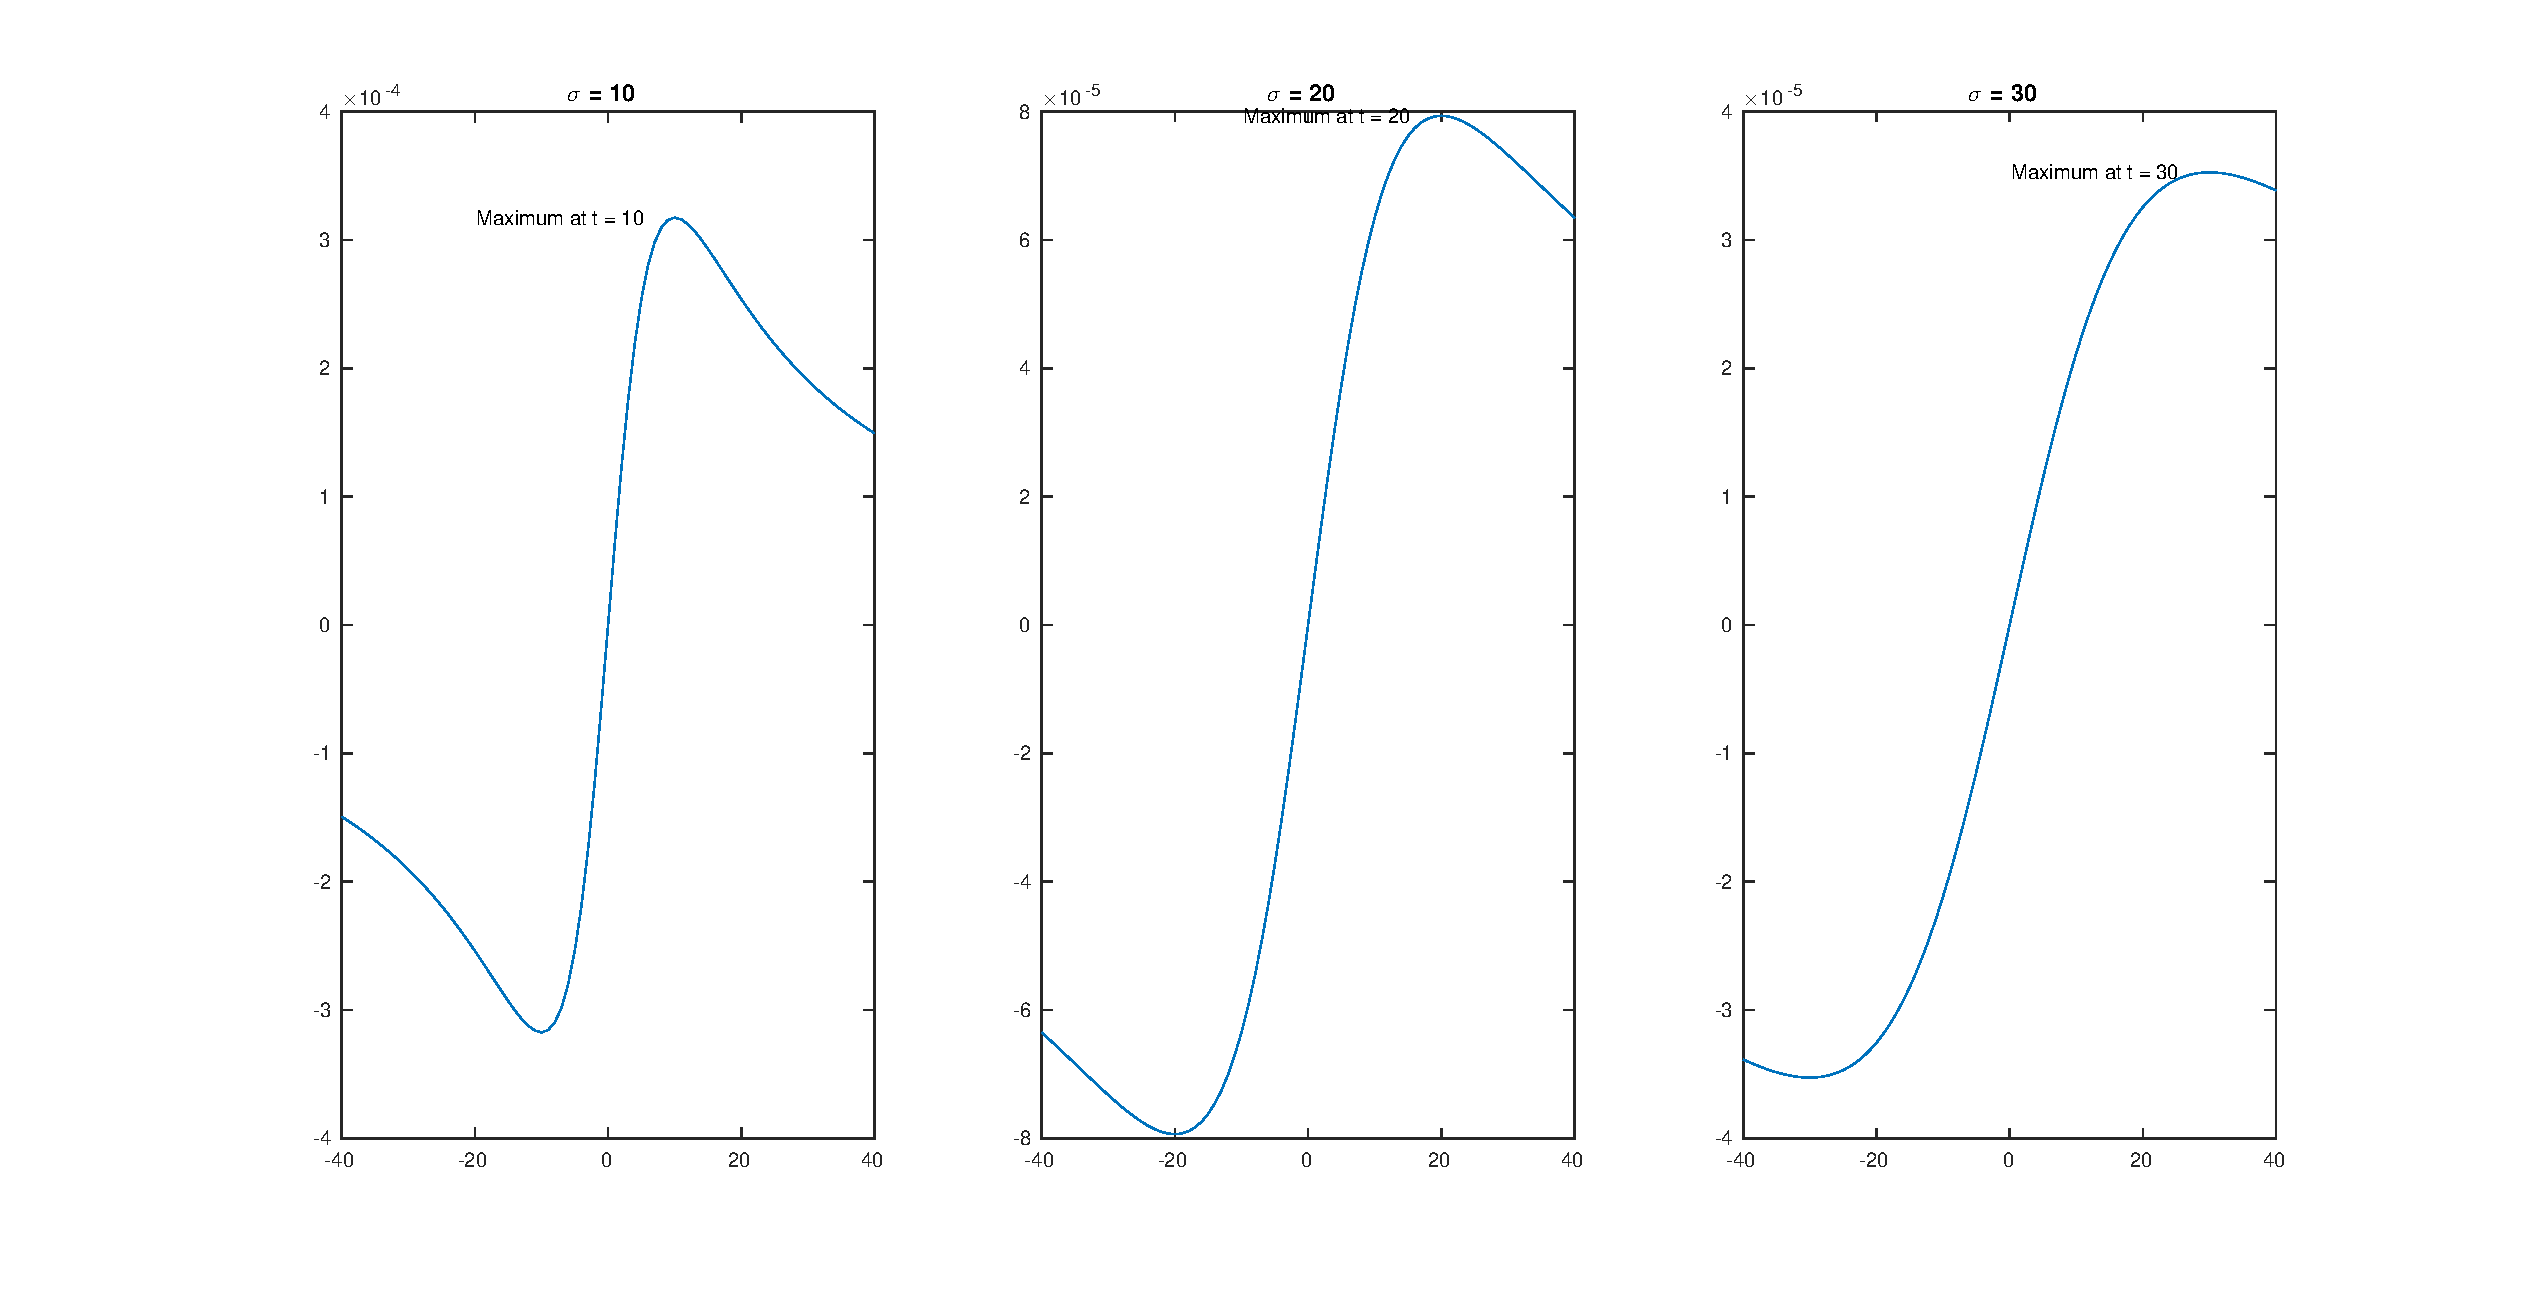
\includegraphics[width=\textwidth]{q3_3.eps}
\caption{Figure the graph for $\dpip\Delta J\dpip^2$ with values $\sigma=\{10,20,30\}$. Along with the graph at what $\tau$-value the maximum if found.}
  \label{q4_4}
\end{figure}
Where we can verify that the maximum is indeed found at $\tau=\sigma$.

\subsection*{(d)}
The procedure is the same as in (d) from question $2$, i.e. looking at values of pixels for scales that are adjacent ($\tau-1, \tau, \tau+1$) to find the best values for $\tau$ . The difference is we locate edges instead of blobs. However, we were not able make it work due to time restraints, which is why we lack the results.

\section*{Question 4}
We can compute the linear shift invariant, as a convolution of the input image $f(x,y)$ and PSF $h(x,y)$ with noise $n(x,y)$ added to it:
$$
  g(x,y) = f(x,y) ** h(x,y) + n(x,y)
$$
The function \texttt{LSI} takes two parameters: An image and a kernel. It then convolves the image with the kernel and adds the given noise, which has been hardcoded as Gaussian noise. The function is seen below:
\lstinputlisting[language=Matlab]{src/LSI.m}
Running the function on the image \texttt{lena.tif} with a gaussian kernel and added gaussian noise produces the right image in Figure \ref{q4_1}. The gaussian kernel uses a window of the same size as the image and has $\sigma=2$.
\begin{figure}[H]
  \centering
  \captionsetup{justification=centering}
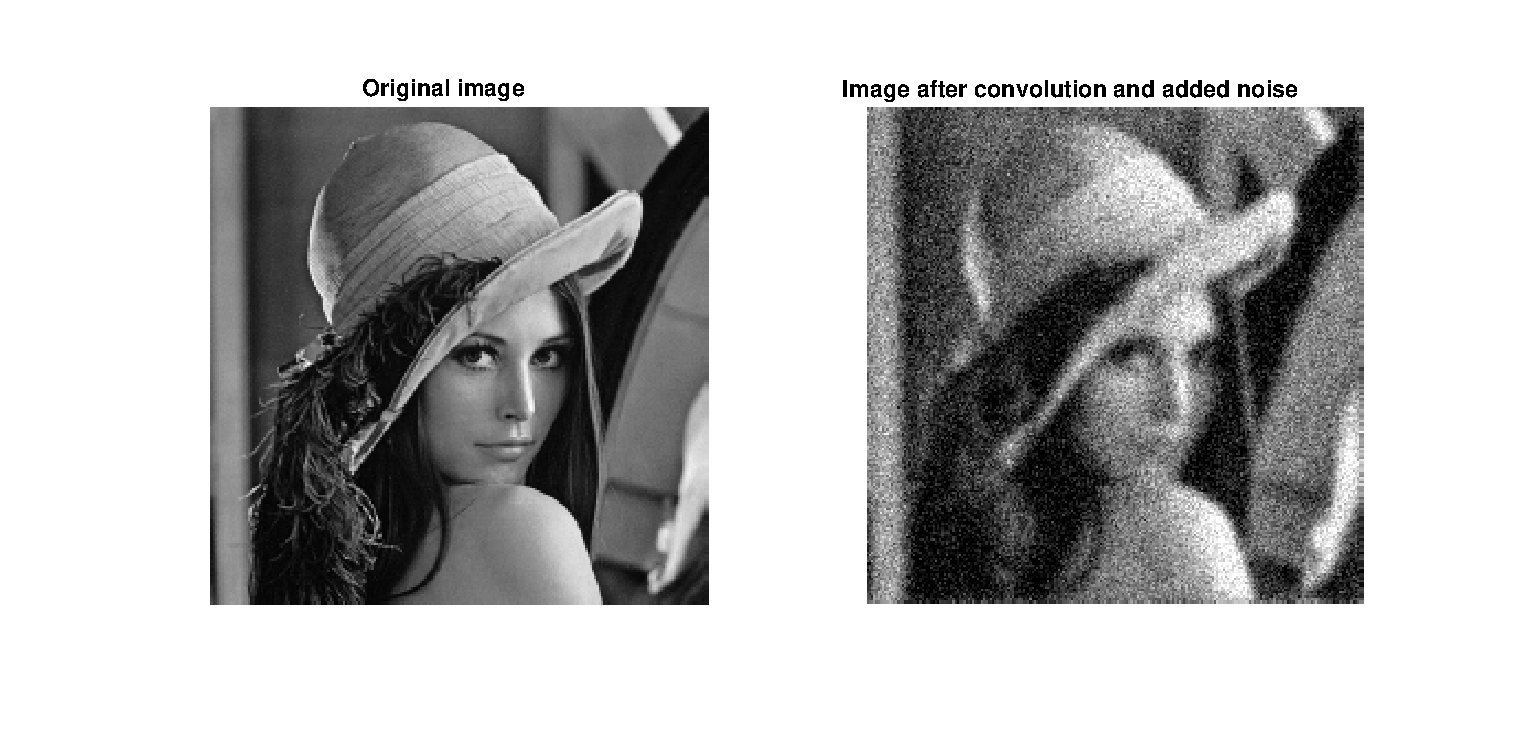
\includegraphics[width=\textwidth]{q4_1.eps}
\caption{Figure showing the original image and the resulting image from convoluting the image \texttt{lena.tif} with a gaussian kernel and then adding gaussian noise.}
  \label{q4_1}
\end{figure}
The linear shift invariantly degraded image is clearly noisy, but the convolution step is a little harder to notice. It is somewhat possible to see that the image has been smoothed a bit (as the convolution should do when using the gaussian kernel), as the edges of e.g. the hat seems to be somewhat blurred.

\section*{Question 5}
Inverse filtering is implemented in the function \texttt{InvFilt.m}, where the noised image is fourier transformed, as well as the PSF being transformed to an OTF. On this OTF, values less than  $10^{-6}$ are disregarded, while all other values are used to create the deconvolution. This is done by dividing the fourier transformed image with the OTF, and since only values where the OTF value is higher than the threshold are used, this division does not cause any problems. The complete
source for the \texttt{InvFilt.m} function can be seen below:
\lstinputlisting[language=Matlab]{src/InvFilt.m}
Using a noisy image created in the same way question 4 results in the following:
\begin{figure}[H]
  \centering
  \captionsetup{justification=centering}
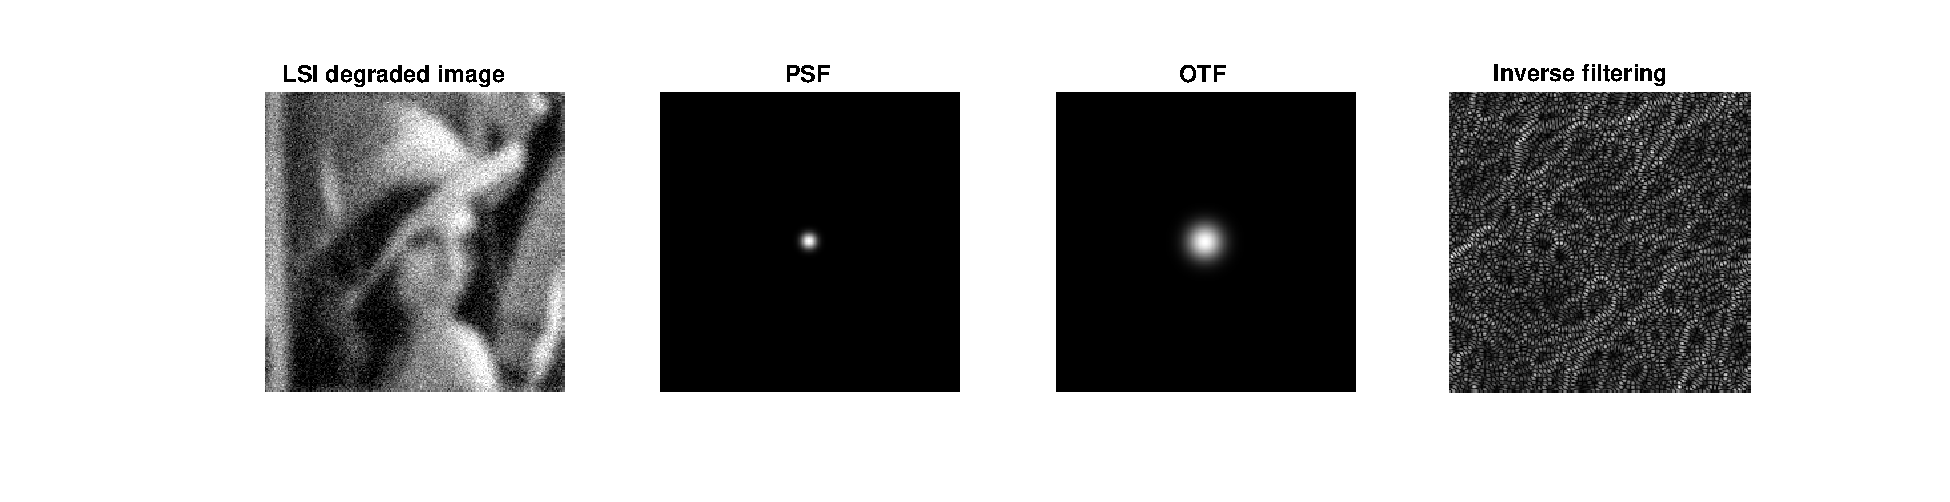
\includegraphics[width=\textwidth]{q5_2.eps}
\caption{Figure showing (from left to right) the LSI degraded image, the PSF used, the transformed OTF and the inverse filtering of the LSI degraded image}
  \label{q5_1}
\end{figure}
It is clearly seen that the resulting image is completely useless, as it doesn’t look anyway like the initial image. This is due to the noise, which the inverse filtering cannot handle.\\

If the inverse filtering is used on convolved images, which hasn’t had any noise added, the  result looks as follows:
\begin{figure}[H]
  \centering
  \captionsetup{justification=centering}
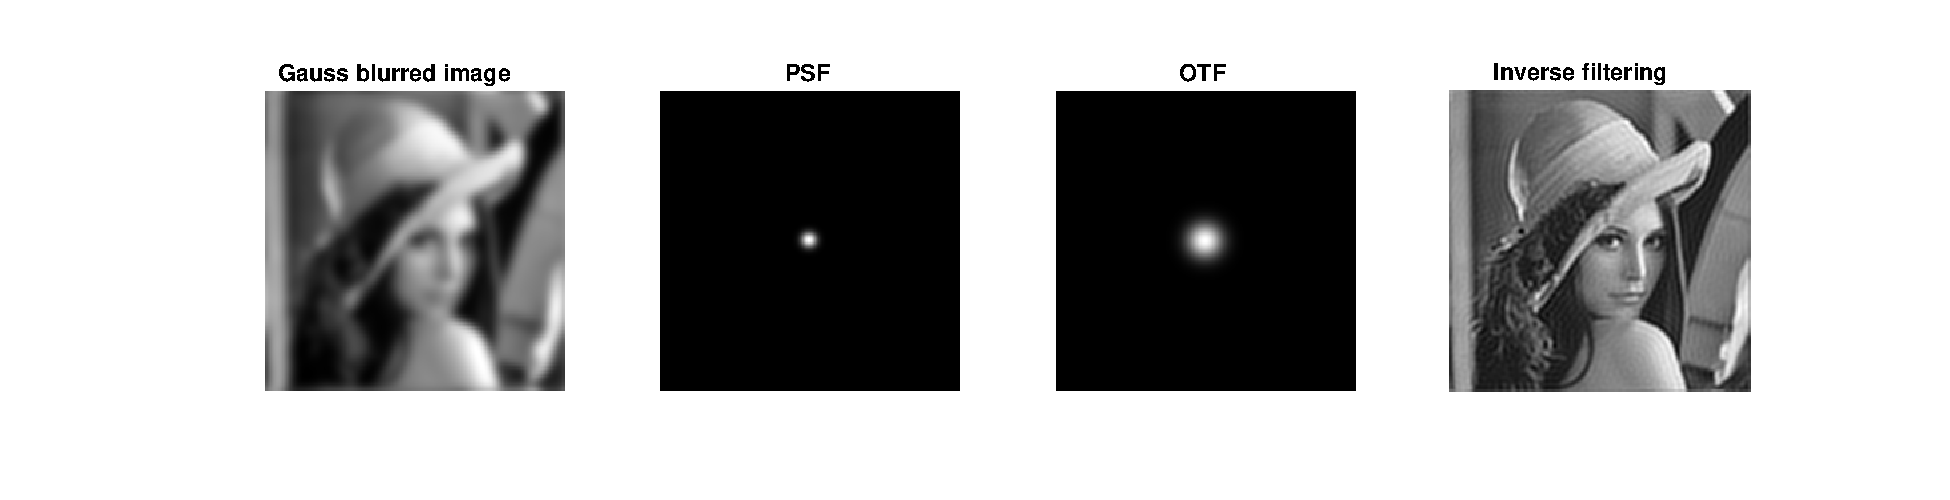
\includegraphics[width=\textwidth]{q5_1.eps}
\caption{Figure showing (from left to right) the Gaussian blurred image, the PSF used, the transformed OTF and the inverse filtering of the Gaussian blurred image}
  \label{q5_2}
\end{figure}
Here, the black border appears since the ‘same’ parameter isn’t applied to the convolution, since no image addition was to be performed afterwards, and thus the resulting size is irrelevant.

However, it can be seen that the inverted image is very similar to the original image, where the blur from the convolved image is removed.
\section*{Question 6}
To overcome the problems with noise from inverse filtering, Wiener filtering attempts to calculate a ratio between how much the image and the noise influences the image for each pixel, and only use the values where the image is most dominant. When doing the filtering, the thresholding can either be done by a constant ratio (e.g. the ratio between the average of the power spectrum of noise and image respectively), or by some autocorrelation. In matlab, Wiener filtering can be done by the function
\texttt{deconvwnr}. Using this yields the following results, where the image to the left is the original image, the image in the middle is the image found using a scalar ratio, while the image to the right is the image found using autocorrelation.
\begin{figure}[H]
  \centering
  \captionsetup{justification=centering}
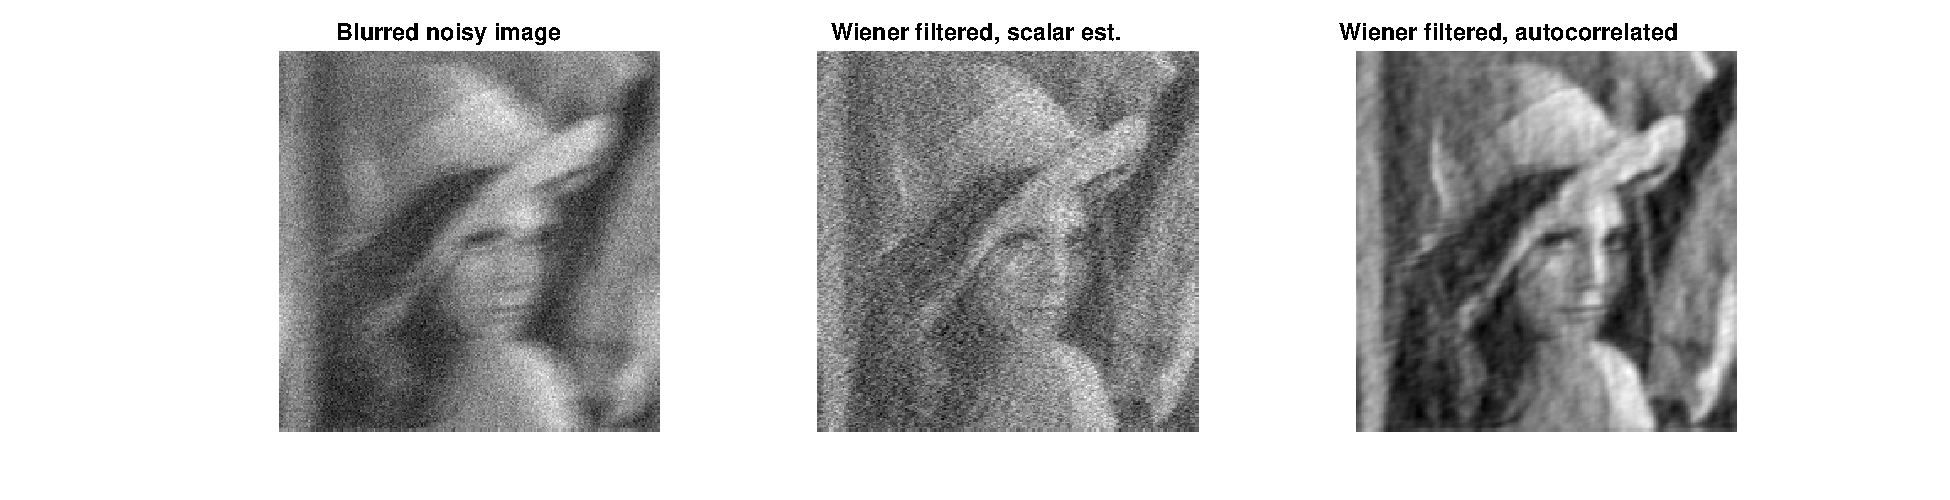
\includegraphics[width=\textwidth]{q6_1.eps}
\caption{Figure showing restoration using two variants of the Wiener filter. (from left to right) blurred image with Gaussian white noise, Wiener filtered image with scalar estimate of total power in noise and signal and Wiener filtered image with autocorrelation of noise and signal provided}
  \label{q6_1}
\end{figure}
From Figure \ref{q6_1} it seems like when the Wiener-filter is applied with the scalar estimate, the details become a little more obvious, although alot of the noise remains. In the autocorrelated image, seems to have removed good deal more noise than of the scalar estimate one. The restored image is far from perfect but represents a significant improvement on the original.

Generally the result seems promising, but we must be remembered that the wiener filtering takes in the realization of the noise, which must be assumed to only rarely be available for noisy images.
\end{document}
